%%%%%%%%%%%%%%%%%%%%%%%%%%%%%%%%
%%%
%%% Research Summary
%%%
%%% Author - Steve Hurder
%%%
%%% Date Started: October 12, 2009
%%% Date Completed: November 15 , 2009
%%%%%%%%%%%%%%%%%%%%%%%%%%%%%%%%[11pt]{amsart}
\usepackage{graphicx}
\usepackage{amssymb}
\usepackage{colortbl}
\usepackage{epstopdf}
\usepackage{url}


\usepackage[top=1in, bottom=1in, left=1in, right=1in]{geometry}

\newcommand{\student}[1]{\vspace{.5cm}\fbox{\parbox{0.95\linewidth}{{\small
        #1}}}\vspace{.5cm}}
\providecommand{\blue}[1]{{\color{blue}{#1}}}
\providecommand{\red}[1]{{\color{red}{#1}}}
\providecommand{\green}[1]{{\color{green}{#1}}}

\begin{document}

 \title{Humans in the Loop for Transparent, Interpretable Machine Learning}

 \author{Jordan Boyd-Graber, University of Maryland}
%\institute{University of Colorado, Boulder CO 80309, USA}


\date{Summer 2022}

\maketitle

Artificial intelligence\footnote{I am taking a fairly broad
  interpretation of what constitutes \abr{ai}; some of my examples
  might be better characterized machine learning.  But rather than
  distracting from the research statement by explicitly delinating the
  boundaries, I'm going to embrace the all-encompassing \abr{ai} and
  instead be as specific as possible in describing the specific tools
  I use.} (\abr{ai}) is ubiquitous: detecting spam e-mails, flagging
  fraudulent purchases, and providing the next movie in a Netflix
  binge.
%
But they do not exist in a vacuum: as \newcite{schneidermann-22}
argues, \abr{ai} will need to exist in a \emph{collaboration} with
humans.
%
My goal is to create metrics to measure whether \abr{ai} methods make
sense to users, building frameworks to explicitly measure the
effectiveness of human--computer teaming, improving computers' ability
to surface information to humans, and to apply \abr{ai}
to applications that help illuminate complex social science
applications.

\section{Evaluating Interpretability}

My journey with evaluating interpretability began over ten years ago
with topic models.
%
Topic
models are sold as a tool for understanding large data collections: lawyers
scouring Nordstream e-mails for a smoking gun, journalists making sense of Wikileaks,
or humanists characterizing the oeuvre of Lope de Vega.
%
But topic models'
proponents never asked what those lawyers, journalists, or humanists
needed.
%
Instead, they optimized \emph{held-out likelihood}. When my colleagues
and I developed the \emph{interpretability} measure to assess whether topic
models' users understood their outputs, interpretability and
held-out likelihood were negatively correlated~\cite{chang-09b}!
%
The topic modeling community (including me) had fetishized complexity
at the expense of usability\dots and topic modeling is not alone,
question answering has distinct but similar issues with
evaluation~\cite{boyd-graber-20}.

\begin{center}
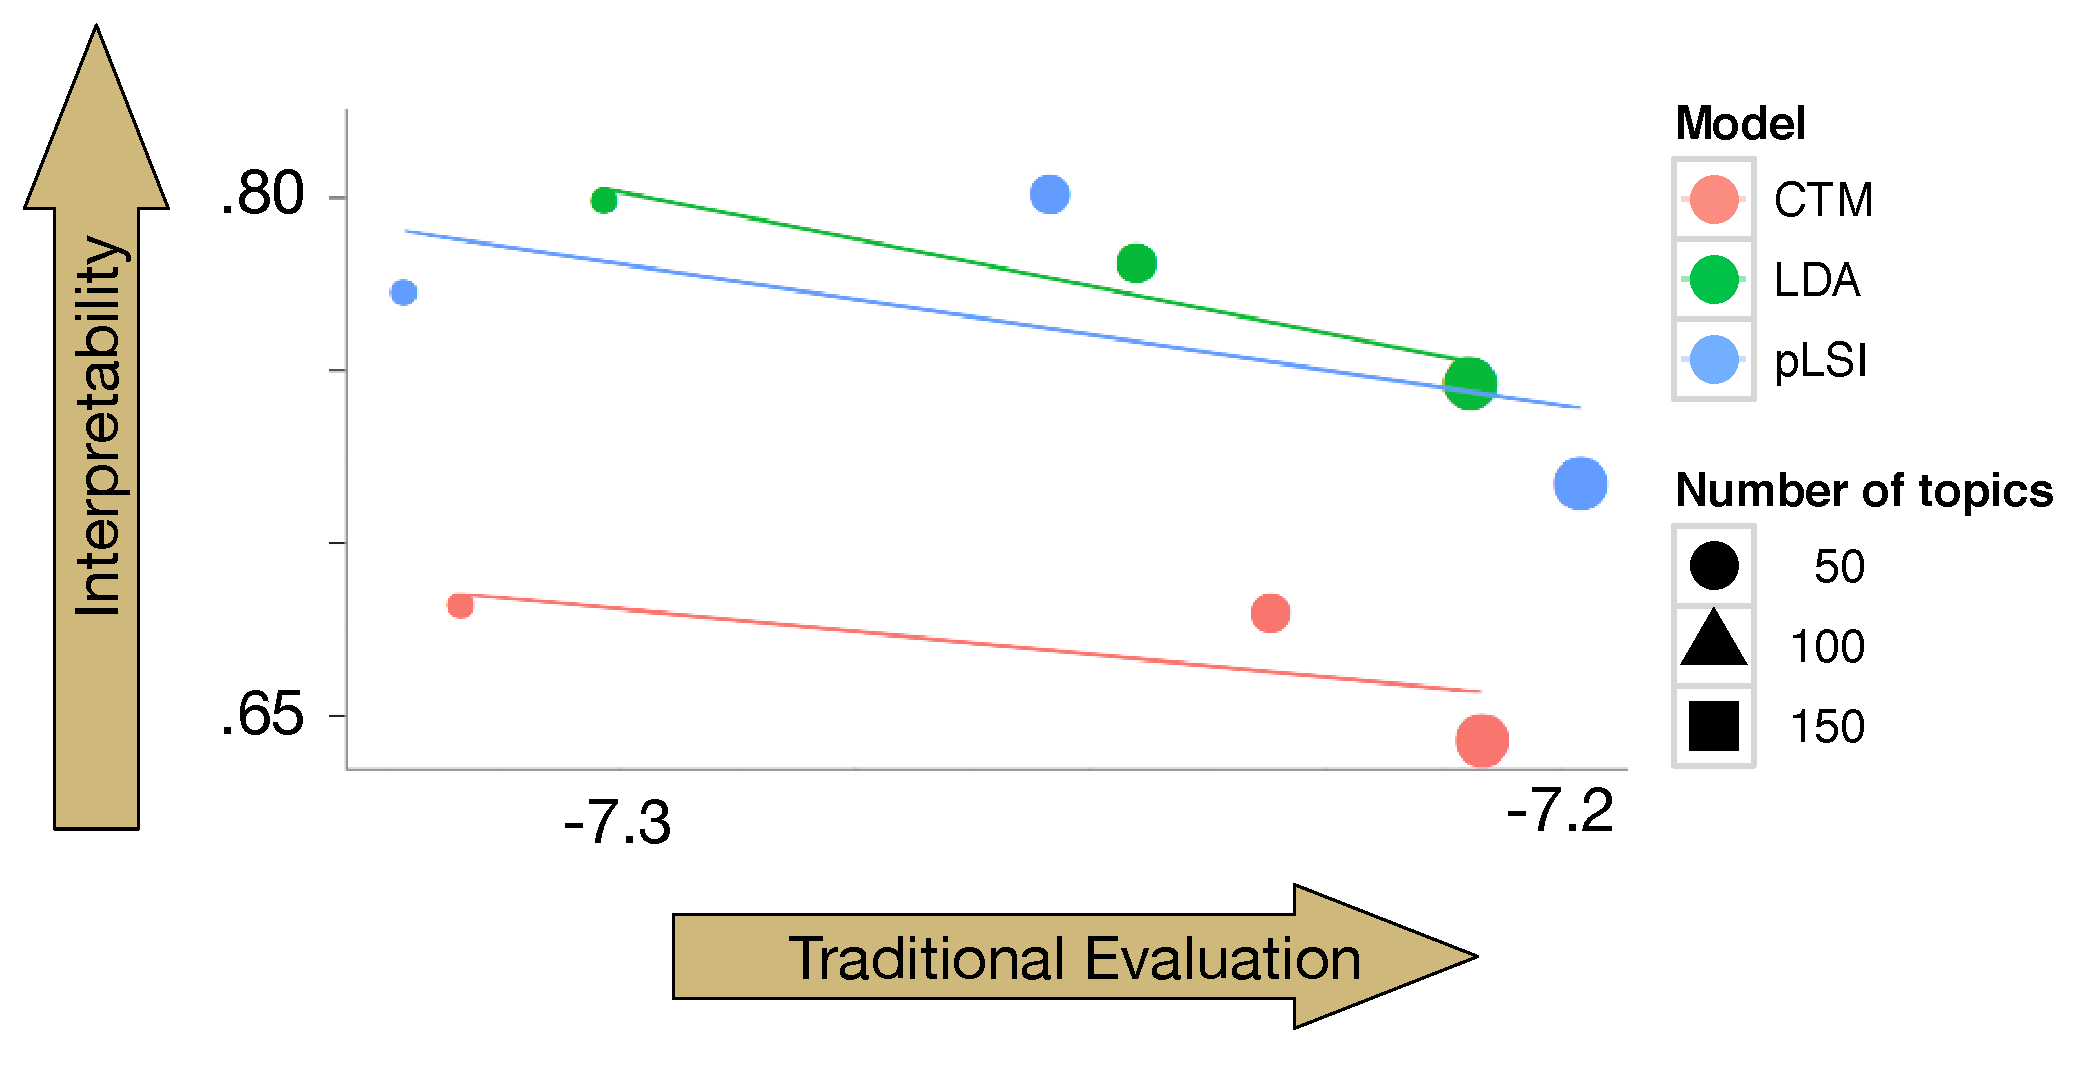
\includegraphics[width=.5\linewidth]{images/prec_ll_4}
\end{center}

Since this humbling discovery, I've built topic models that are a collaboration
between humans and computers.  The computer starts by proposing an organization
of the data.  The user separates confusing clusters or joins
similar clusters together~\cite{hu-14:itm}.  The model updates and directs the user to
problematic areas that.  This is a huge improvement over the
``take it or leave it'' philosophy of most machine learning algorithms.

Focusing on collaboration also requires algorithms that are low
latency (not just high throughput).  We developed methods that go
beyond traditional proababilistic interpretations. We extend the
geometric interpretations of admixture models developed by Arora et
al.~\cite{arora-12} to multi-anchor topics~\cite{lund-17} and
multi-lingual topics~\cite{Yuan-18}. We have also developed better
understanding of projection-based multilingual representations via
graph theory~\cite{Fujinuma-19} and the convergence of alternating
projections~\cite{Zhang-19}.

After we proposed our ``reading tea leaves'' evaluation, it's heartening that \newcite{lau-14} and their ``machine reading tea leaves''
(which correlate with our human measures) have become a standard topic
model evaluation.\footnote{E.g., in a survey of N modern neural topic
  modeling papers, X\% use the tea leaves evaluation.}
%
However, as we argue in \newcite{hoyle-21}, you cannot just use this
evaluation forever and forget about humans.
%
As topic models evolve (e.g., incorporating
neural components), you need to validate that these automatic metrics
still correlate with wether it is useful for a human--computer
collaboration.
%
In other words, automatic metrics are not a replacement for actually
evaluating a human gaining understanding about a corpus (E.g., the
label induction task we proposed in \newcite{poursabzi-17}).

\section{Teaming as an Evaluation}

Within the \abr{hci} community, we have argued for the foundations of
what should go into human--computer teams: computers that incorporate
users suggestions~\cite{kumar-19}; explanations with
accountability~\cite{smith-20}; and stabile
explanations~\cite{smith-20:adherence}.

In addition to these human-centered understanding of users' needs and
desires, we've developed machine learning approaches to measure how
well users complete a task.
%
For example, for a question answering task, we measured how much the
accuracy of the human--computer \emph{team} increases with different
explanations.
%
With this, we uncovered that users' stated preferences don't always
align with helps the most at a task: users like seeing confidence but
this is not the most important explanation of \abr{ai} decision
making.
%
Moreover, it also shows that crowdworkers need very different tools in
a human--computer collaboration than experts~\cite{feng-19}: experts have much higher
accuracy and can handle much more detailed explainations without being
overloaded.

\section{Question Answering and Machine Translation}

However, building collaborations between humans and computers also
sometimes requires innovation in how the underlying approaches work.
%
Here, I briefly describe some of the advances that we've made in 
underlying natural processing algorithms.
%
Nearly all of the work here is in collaboration with my colleague Hal Daum\'e at the University of Maryland, much of it in the context of a \abr{nsf} grant where I served as \abr{pi}.
%
This grant  argued that an  isomorphism between the  ``gold standard''
trivia format for question  answering and real-time translation offers
opportunities  for  new  \abr{ai}  techniques  that  can  address  the
word-by-word properties of both problems.

Like many researchers, I had to make the transition from statistical models to neural models.
%
I was fortunate to have Mohit Iyyer to help drag me kicking and screaming into modernity.
%
As an exercise in proving to me that the nonlinearities of neural
methods were useful, we developed the deep averaging network~\cite{}, an
incredibly simple model that is still being used even in the age of
transformers~\cite{}.

Likewise, in quesiton answering we have proposed new evaluation
mechanisms for knowing if an answer is correct~\cite{si-21} or to
improve unsupervised retrieval of information to answer complicated
questions~\cite{zhao-20}.
%
For these complicated questions, you also need to be able to
incorporate feedback when the system gets it wrong, as my former
student did in \newcite{}, building on our previous work for tabular
question answering~\cite{} and question answering over discourse
chains~\cite{}.

We also introduced reinforcement learning to \emph{simultaneous
  machine interpretation}~\cite{Grissom:He:Boyd-Graber:Morgan-2014}, a
  language-based task that requires significant human intuition,
  insight, and---for those who want to become
  interpreters---training. Because verbs end phrases in many
  languages, such as German and Japanese, existing algorithms must
  wait until the end of a sentence to begin translating (since English
  sentences have verbs near the start). We learned tricks from
  professional human interpreters---passivizing sentences and guessing
  the verb---to translate sentences sooner~\cite{He-15}, letting
  speakers and algorithms cooperate together and enabling more natural
  cross-cultural communication.  We can also use reinforcement
  learning to learn machine translation feedback from noisy
  supervision such as star ratings on a webpage~\cite{nguyen-17}.

This framework---using reinforcement learning to capture human
strategies---was featured in Liang Huang's \abr{acl} keynote and helps
build metrics that can support human--computer collaborations.
%
While we would not trust a computer to take over a sensitive
negotiation at the \abr{un} or the \abr{eu}, but it might well make
sense for instead of two human interpreters who alternate active
translation (the norm for high-stakes negotiation), we can augment a
single interpreter with a computer assistant, cooperating to translate
challenging text.

\section{Connecting with Social Science: Pedagogy, Framing, and Deception}

The reverse of cooperation is competition; it also has much to teach computers.
%
Following the pattern of looking at trivia games, I've increasingly looked at language-based games whose clear goals and
intrinsic fun speed research progress.
%
For example, in \emph{Diplomacy}, users
chat with each other while marshaling armies for world conquest. Alliances are
fluid: friends are betrayed and enemies embraced as the game develops. However,
users' conversations let us predict when friendships break: betrayers writing
ostensibly friendly messages before a betrayal become more polite, stop talking
about the future, and change how much they write~\cite{niculae-15} in follow-on
work, we develop a dataset that helps predict both when users lie to each other
and when recipients of lies detect deception~\cite{Peskov-20}.
%
Diplomacy may be
a nerdy game, but it is a fruitful testbed to teach computers to understand
messy, emotional human interactions.
%
We are continuing to look into these questions with researchers from
across the nation in a new \abr{darpa} program: \abr{shade}, which focuses
on the game that were were first to highlight for its linguistic deception as a computational task.

A game with higher stakes is politics. However, just like Diplomacy, the words
that people use reveal their underlying goals; computational methods can help
expose the ``moves'' political players can use. With collaborators in political
science, we've built models that: show when politicians in debates
strategically change the topic to influence others~\cite{nguyen-12,Nguyen-14b};
frame topics to reflect political leanings~\cite{nguyen-13:shlda}; use subtle
linguistic phrasing to express their political leaning~\cite{iyyer-14a}; or
create political subgroups with larger political
movements~\cite{Nguyen:Boyd-Graber:Resnik:Miler-2015}.

Because political discourse is built on a common set of commonly
accepted facts, we have focused on developing fact checking: datasets
for general knowledge fact checking~\cite{eisenschlos-21} and climate
change fact checking~\cite{20-diggelmann}.
%
However, because fact checking is part of an information arms race, we
need to build these examples as part of a human-in-the-loop
adversarial process.

\section{Human-in-the-Loop Adversarial Examples}

One of the most fun aspects of my research has been building
trivia-playing robots~\cite{boyd-graber-12,iyyer-14b,iyyer-15}; in
addition to the research, it has faced off against
former Jeopardy champions in front of hundreds high school
students.\footnote{\url{https://www.youtube.com/watch?v=LqsUaprYMOw}}
%
But after defeating some of the smartest trivia players, did I
actually believe that our system was better at question answering?
%
No!

Adversarial examples first came out of the vision community: add a
small epsilon to an example and suddenly a object detector calls a
turtle a gun.\footnote{Point of personal pride: I mentored Kevin on
another previous research project but had nothing to do with this later
adversarial work.}
%
While others have attempted to create eadversarial examples for
language using paraphrasing, it's hard to know if the changes are
perceptually negligable and it's hard to ``add epsilon'' to a discrete
word.

Consistent with the theme of my research, my \abr{nsf career} grant
proposed to have a human in the loop.
%
With Eric Wallace, and undergraduate student, we built a system that
could help an expert trivia question writer to stump a computer: as
the author writes the question, it shows the author what the system is
thinking~\cite{wallace-18}.
%
And it worked, even generalizing across types of
models~\cite{wallace-19}.
%
Meta Facebook adopted this human-in-the-loop framework with
gusto~\cite{bartolo-20} in their Dynabench framework and the Dynamic
Adversarial Data Collection workshop.

\section{Future Work}

I recently outlined how we can improve measurement of question
answering progress~\cite{boyd-graber-20}.
%
One critical component is going beyond raw accuracy, creating multivariate measures of when computers are doing well.
%
\newcite{rogers-22} has a clear ontology of what skills a computer answering questions \emph{should} posess, and we have measurement tools to compare human and computer abilities at question answering~\cite{rodriguez-21}.
%
But we lack the appropriate datasets to effectively probe if computers possess these skills.  

Thus, we are building new question answering datasets that honestly reveal a computer's skils, working with the \textit{Online Quiz League} where the competition is not to answer trivia questions but to ask challenging questions that illuminate a computer's weaknesses.
%
At the same time, we're also working to improve the representation of these datasets.
%
Google's Natural Questions, SQuAD, and others all are overwhelmingly male and either American on British~\cite{gor-21}.

I am also working with educators to deploy these techniques to better
measure students' knowledge: if our representations can capture what
makes a question hard, it can order a \emph{curriculumn} to help a
student learn the material.

\section{Future Work}

%% \vspace{12cm}

%%  \parbox{\linewidth}{I certify that this
%%   statement is a current and accurate statement of my
%%   professional record to the best of my
%%   knowledge \flushright  
\includegraphics[width=.2\linewidth]{resume_src/signature} \\
%% \flushright  (\today{})}

\clearpage

%%%%%%%%%%%%%%%%%%%%%%%%%%%%%%%%

\bibliographystyle{resume_src/splncs03}

\begin{center}
Full list of  three book chapters, eleven journal publications, and eighty-five conference
publications at \url{http://boydgraber.org/dyn-pubs/year.html}
\end{center}

%\bibliographystyle{unsrtnat}
\bibliography{resume_src/journal-full,resume_src/jbg}
\noindent\rule{4cm}{0.4pt}
\end{document}
